\documentclass[10pt]{article}

\usepackage[a4paper,top=2.65cm,bottom=3.4cm,left=2.5cm,right=2.5cm]{geometry}
%\usepackage[T1]{fontenc}		%implementa nei font gli accenti (crea un casino facendo tutto pixellato)
\usepackage[utf8]{inputenc}		%importa i caratteri utf
\usepackage{inputenc}
\usepackage[italian]{babel}
\usepackage{amsmath,amssymb}	%per visualizzare la matematica (per text{})
%\usepackage{graphicx}			%per le figure
\usepackage{xcolor}				%per scrivere colorato XCOLOR per lstlisting colorato (se non c'è tikz)
\usepackage[toc,page]{appendix}	%per l'implementazione delle appendici
%\usepackage{subfig}				%per figure multiple in una stessa figure
%\usepackage{pdfpages}			%per includere pezzi di pdf
\usepackage{float}				%per mettere le figure nel posto giusto
\usepackage{tikz}				%per le immagini vettoriali da LateX
\usepackage{listings} 			%Per inserire codice
\usepackage{pxfonts}			%per il bold nei lstlisting
%\usepackage{scrextend}			%per labeling
\usepackage[inline]{enumitem}	%per l'itemize senza spazi [noitemsep]
\usepackage{footnote}			%per più note nella tabella (ambiente "savenotes")


\definecolor{mymauve}{rgb}{0.58,0,0.82}
\lstset { %
    language=MATLAB,
    backgroundcolor=\color{black!5}, % set backgroundcolor
    basicstyle=\footnotesize\ttfamily, % basic font setting
    frame=shadowbox,
    breaklines= true, % va a capo automatico
    numbers=left, % numera le righe
    commentstyle=\color{gray}, % commenti grigi
    stringstyle=\color{mymauve}, % string literal style
    numberstyle=\footnotesize\ttfamily, %formato dei numeri a lato delle righe
    keywordstyle=\color{black}\bfseries, % style for keywords
}




\begin{document}


\title{\Huge{\textbf{MchiN strisce}}\\ \Large{programma di analisi delle sezioni a strisce}}
\author{Andrea Marchi}

\maketitle

\begin{center}
\begin{Huge}
\textcolor{red}{QUESTO DOCUMENTO NON É ANCORA COMPLETO}
\end{Huge}
\end{center}

\tableofcontents

\newpage




\section{Programma}

Il programma consiste in una classe (\texttt{MchiNstrisce}) implementata in \textit{MATLAB}. Basta inserire il file corrispondente alla definizione della classe (il file "\texttt{MchiNstrisce.m}") nella cartella del file che la chiama, o in una delle sottocartelle nel \textit{path} di MatLab per utilizzare la classe e tutte le sue funzionalità.

\subsection{Teoria di base}

L'analisi a fibre consiste nel dividere la sezione in "piccole" aree chiamate \textit{fibre}\footnote{\textcolor{red}{Riferimento al modello di Drukcer}}. Le \textit{strisce}, usate in questa classe come discretizzazione delle sezioni, non sono altro che fibre larghe quanto la larghezza della sezione ad una determinata $y$ (secondo l'asse perpendicolare all'asse di sollecitazione)\footnote{In questo caso l'asse di sollecitazione è l'asse $y$ e quindi la larghezza della fibra $i$-esima è la larghezza complessiva della sezione (per quel determinato materiale) all'"altezza" $y_i$ della fibra.}.

\begin{figure}[H]
\centering
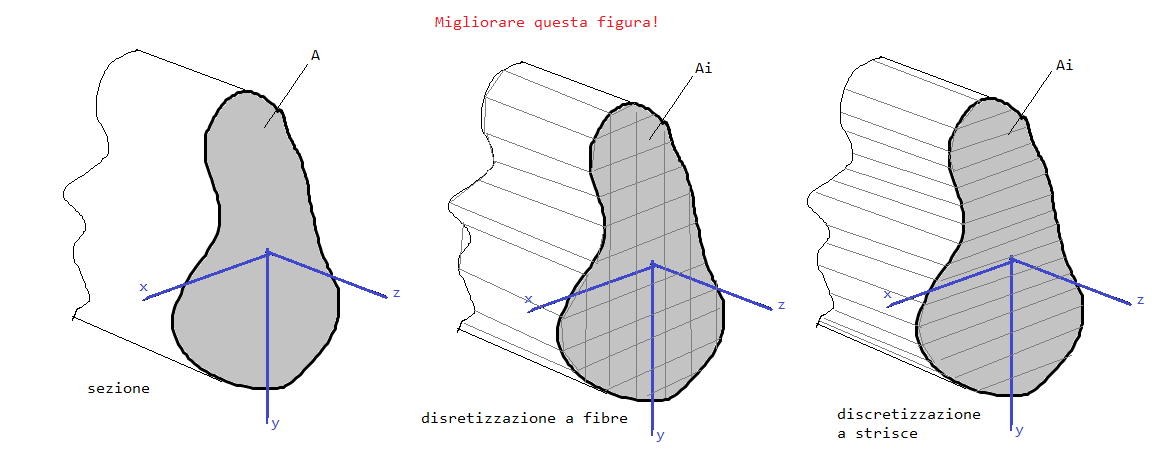
\includegraphics[width=\textwidth]{img/discretizzazione_sezione.png}
\caption{\footnotesize Discretizzazione della sezione in \emph{fibre} e in \emph{strisce}.}
\end{figure}
\textcolor{red}{in realtà la y l'ho presa verso l'ALTO io (il contrario della convenzione italiana}

Le equazioni che definiscono le caratteristiche di sollecitazione interne ad un elemento, a partire dalle tensioni interne al continuo, sono:
\begin{equation}
N_{int}(z) = \int_A \sigma_z(x,y,z) \; dA 
\qquad \qquad
V_{int}(z) = \int_A \tau_{zy}(x,y,z) \; dA
\qquad \qquad
M_{x,int}(z) = \int_A \sigma_z(x,y,z) \; y \; dA
\end{equation}
dove gli integrali sono integrali superficiali svolti sulla sezione della trave (nel piano $xy$). Dato che in generale la forma della sezione (e quindi il dominio di integrazione) non è esprimibile in forma analitica in funzione di $x$ e $y$, si ricorre alla discretizzazione della sezione in elementi piccoli (ma non infinitesimi) approssimando gli integrali in somme.
Tale discretizzazione permette di calcolare anche sezioni costituite da materiali eterogenei e con legami costitutivi non-lineari (come il calcestruzzo armato).
\begin{equation}
N_{int} = \sum_i \sigma_z(x_i,y_i) \; A_i 
\qquad \qquad
V_{int} = \sum_i \tau_{zy}(x_i,y_i) \; A_i
\qquad \qquad
M_{x,int} = \sum_i \sigma_z(x_i,y_i) \; y_i \; A_i
\end{equation}
dove $x_i$ e $y_i$ sono le coordinate del baricentro della fibra (sempre rispetto al baricentro della sezione omogeneizzata $G$). Inoltre la coordinata $z$ è stata omessa in quanto si è interessati a valutare la resistenza della sezione, che generalmente non varia al variare della lunghezza dell'elemento.

\begin{center}
\textcolor{red}{immagine di una sezione piana discretizzata con le quote di $b_i$ con vari materiali e anche dei buchi per mostrare le varie opportunità}
\end{center}

L'ipotesi principale utilizzata nel calcolo delle azioni interne è che \emph{le sezioni piane e perpendicolari all'asse dell'elemento rimangono piane e perpendicolari anche nella configurazione deformata}.
Dunque l'analisi della sezione a fibre consiste nel determinare le azioni interne ($N_{int}$, $V_{int}$ e $M_{x,int}$) in funzione della deformazione, tramite i legami costitutivi dei vari materiali. Fare questo calcolo in maniera numerica per ogni striscia permette di utilizzare anche legami costitutivi non-lineari, che risulta particolarmente conveniente per elementi in calcestruzzo armato dove il comportamento non-lineare è predominante.
Per trovare la deformazione corrispondente ad un determinato sistema di azioni esterne ($N$, $V$, e $M_x$) si utilizzano le equazioni di equilibrio\footnote{Da notare che, in generale, le equazioni di equilibrio impongono che la somma delle forze e dei momenti devono essere uguali a zero
\begin{equation}
\text{equilibrio alla traslazione:} \rightarrow \sum \mathbf{f}_i = \mathbf{0}
\qquad \qquad
\text{equilibrio alla rotazione:}   \rightarrow \sum \mathbf{m}_i = \sum \mathbf{f}_i \times \mathbf{d}_i = \mathbf{0} 
\end{equation}
In questo caso tuttavia le azioni interne sono da considerarsi come delle \emph{reazioni}. Dunque la condizione di equilibrio è un'eguaglianza tra azioni ($N$, $V$, e $M_x$) e reazioni ($N_{int}$, $V_{int}$ e $M_{x,int}$).}
\begin{equation}
N_{int} = N
\qquad \qquad
V_{int} = V
\qquad \qquad
M_{x,int} = M_x
\end{equation}
insieme ad algoritmi di soluzione per problemi non-lineari. Gli algoritmi presi in considerazione in questa trattazione sono l'algoritmo di \emph{bisezione} e quello di \emph{Newton-Raphson}.



\subsection{Geometria della sezione}



\subsection{Situazioni limite}

\textcolor{red}{Grafico $M-\chi$ in cui sono mostrati i punti limite: Punto di primo snervamento, snervamento e rottura}



\subsection{Punto di fessurazione}

La fessurazione avviene quando la fibra più allungata supera l'allungamento di rottura del calcestruzzo $\varepsilon_{ct}$. Per calcolare correttamente le azioni interne nel punto di fessurazione bisogna utilizzare un legame costitutivo per il calcestruzzo che includa la descrizione del comportamento a trazione.

\begin{figure}[H]
\centering
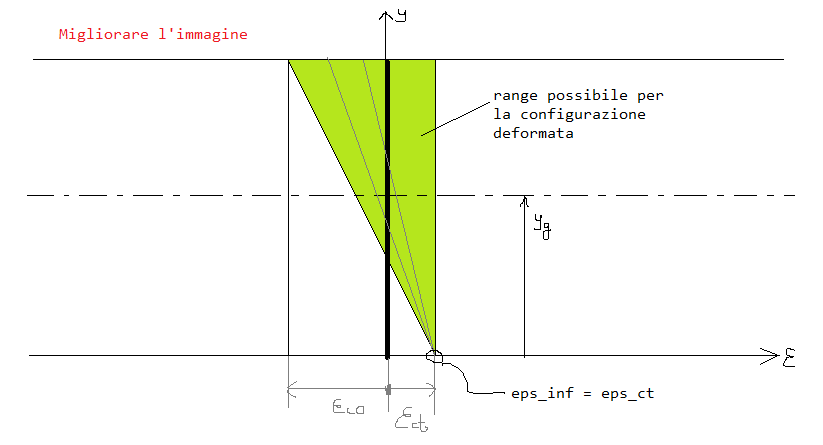
\includegraphics[width=0.8\textwidth]{img/punto_fessurazione.png}
\caption{\footnotesize Intervallo possibile per la configurazione deformata nella condizione di prima fessurazione.}
\end{figure}


\subsubsection{Punto di snervamento}

\begin{figure}[H]
\centering
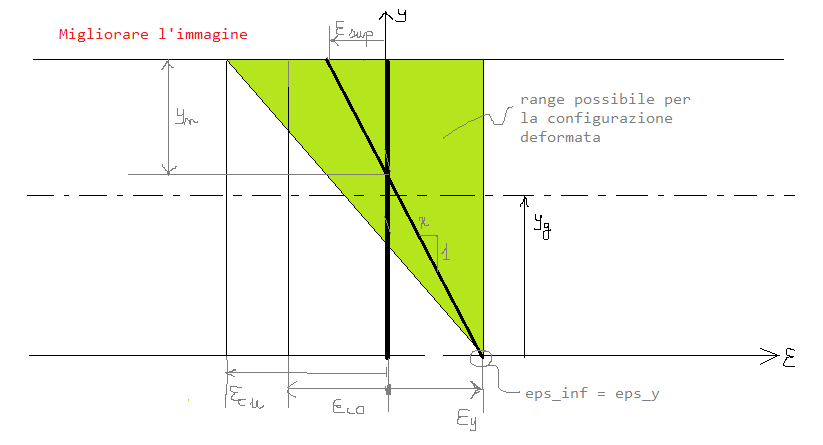
\includegraphics[width=0.8\textwidth]{img/punto_snervamento.png}
\caption{\footnotesize Intervallo possibile per la configurazione deformata nella condizione di snervamento.}
\end{figure}


\subsubsection{Punto di rottura}

La \emph{rottura} di una sezione si raggiunge quando il \textit{calcestruzzo (o l'acciaio) raggiunge la sua deformazione ultima}.

Dato che, secondo l'ipotesi cinematica principale, \textit{le sezioni piane rimangono piane} il campo di deformazione della sezione è definito da due parametri. Dunque, definiti dei legami costitutivi per il calcestruzzo e l'acciaio, anche le azioni interne $N_{int}$ e $M_{int}$ dipendono da due parametri. In questo particolare caso risulta conveniente prendere come parametri la deformazione al lembo inferiore $\varepsilon_{inf}$ e la deformazione al lembo superiore $\varepsilon_{sup}$. La deformazione, in funzione della profondità $y$, è definita da
\begin{equation}
\varepsilon(y;\varepsilon_{inf},\varepsilon_{sup}) = \frac{\varepsilon_{sup}-\varepsilon_{inf}}{H} \; y + \varepsilon_{inf}
\end{equation}

\begin{center}
\textcolor{red}{Immagine con la deformazione nel piano $yz$ e anche la sezione\\ affianco con la fibra messa in evidenza}
\end{center}

Dunque lo gli sforzi interni sono
\begin{align}
N_{int}(\varepsilon_{inf},\varepsilon_{sup}) & = \sum_i \sigma_{cls}[\varepsilon(y_i;\varepsilon_{inf},\varepsilon_{sup})] \; A_i + \sum_j \sigma_{acc}[\varepsilon(y_j;\varepsilon_{inf},\varepsilon_{sup})] \; A_j \\
M_{int}(\varepsilon_{inf},\varepsilon_{sup}) & = \sum_i \sigma_{cls}[\varepsilon(y_i;\varepsilon_{inf},\varepsilon_{sup})] \; y_i \; A_i + \sum_j \sigma_{acc}[\varepsilon(y_j;\varepsilon_{inf},\varepsilon_{sup})] \; y_j \; A_j
\end{align}
dove sono stati esplicitati i contributi delle armature $j$. In generale si possono definire quanti materiali si desiderano, con i relativi legami costitutivi.

La condizione di rottura vincola una delle due incognite. Infatti, se si ha una rottura lato calcestruzzo, la deformazione superiore deve essere pari alla deformazione ultima del calcestruzzo $\varepsilon_{sup} = \varepsilon_{cu}$. In caso di rottura lato acciaio la deformazione del lembo inferiore è pari alla deformazione ultima dell'acciaio $\varepsilon_{inf} = \varepsilon_{su}$. \textcolor{red}{Questo comporta che la flessione nelle sezioni analizzate è sempre presa \textit{positiva}, ovvero che tende le fibre inferiori. Nel caso di flessione negativa il superiore si "inverte" con l'inferiore}.
Una volta fissata una delle due incognite, $\varepsilon_{sup}$ o $\varepsilon_{inf}$ in caso si ha rispettivamente una rottura lato calcestruzzo o lato acciaio, la seconda è trovata grazie all'equazione di equilibrio alla traslazione assiale $N_{int}(\varepsilon_{inf},\varepsilon_{sup}) = N$, dove $N$ è lo sforzo assiale a cui è soggetta la sezione.

Ponendo, per esempio, che la rottura avvenga lato calcestruzzo e quindi, per un momento agente positivo (che comprime le fibre superiori), si ha $\varepsilon_{sup} = \varepsilon_{cu}$ dove si ricorda che ha un valore negativo perché di \emph{accorciamento}. Allora in questo particolare caso si vuole trovare $\varepsilon_{inf}$ invertendo l'equazione di equilibrio
\begin{equation}
N_{int}(\varepsilon_{inf},\varepsilon_{sup}=\varepsilon_{cu}) = N
\end{equation}
Dato che si tratta di un'equazione non-lineare per invertirla si necessita di un metodo di soluzione numerico adatto. In questo caso si utilizza l'algoritmo della \textit{bisezione}. Tale algoritmo consiste nel trovare un range di variabilità del parametro in esame (in questo esempio $\varepsilon_{inf}$) e successivamente riduce tale intervallo in base alla valutazione dell'equazione in esame nei punti estremi ed in quello intermedio. \textcolor{red}{Spiegare meglio in una appendice, oppure mettere un riferimento Pro}.
Come intervallo iniziale per la variabile ricercata si prende
\begin{equation}
\varepsilon_{cu} \leq \varepsilon_{inf} \leq \varepsilon_{su}
\end{equation}
\begin{lstlisting}
eps_infN = eps_cu; %limite inferiore dell'intervallo (negativo: accorciamento)
eps_infP = eps_su; %limite superiore dell'intervallo (positivo: allungamento)
\end{lstlisting}
in quanto, in qualunque caso, non può essere fuori da tale intervallo (altrimenti saremmo in una condizione post-critica e quindi non più in un punto di rottura).
Il valore dello sforzo normale agente $N$ (negativo di compressione) sarà sicuramente compreso tra i valori dello sforzo normale interno $N_{int}$ calcolato nei due punti estremi dell'intervallo
\begin{equation}
N_{int}(\varepsilon_{inf,N},\varepsilon_{sup}=\varepsilon_{cu}) 
\leq N \leq
N_{int}(\varepsilon_{inf,P},\varepsilon_{sup}=\varepsilon_{cu}) 
\end{equation}
La procedura della \emph{bisezione} consiste nel determinare lo sforzo normale in un punto intermedio tra i due
\begin{equation}
\varepsilon_{inf,M} = \frac{\varepsilon_{inf,N} + \varepsilon_{inf,P}}{2}
\end{equation}
ed aggiornare l'intervallo prendendo questo punto intermedio come estremo e quindi \textit{dimezzare} l'intervallo di ricerca\footnote{Proprio per il fatto che ad ogni iterazione l'intervallo di ricerca si dimezza questo metodo è chiamato \emph{metodo di bisezione}.}. La decisione su quale dei due estremi (inferiore o superiore) deve assumere il valore medio dipende dal valore della funzione da risolvere nel punto medio. In particolare se $N_{int}(\varepsilon_{inf,M},\varepsilon_{sup}=\varepsilon_{cu})<N$ allora vuol dire che il valore medio è il nuovo limite inferiore ($\varepsilon_{inf,N} = \varepsilon_{inf,M}$) poiché questo permette di mantenere lo sforzo normale agente $N$ all'interno dell'intervallo di ricerca. Al contrario, se $N_{int}(\varepsilon_{inf,M},\varepsilon_{sup}=\varepsilon_{cu})>N$ allora il valore medio è il nuovo limite superiore ($\varepsilon_{inf,P} = \varepsilon_{inf,M}$).

\begin{center}
\textcolor{red}{inserire una immagine di uno step di bisezione per rendere tutto più chiaro (anche con il riferimento della sezione affianco)}
\end{center}

Tale procedura di dimezzamento dell'intervallo viene ripetuta finché i due estremi non convergono ad un valore, che risulta essere il risultato cercato. Nel caso in cui lo strumento di calcolo possiede una precisione infinita e vengono eseguite infinite iterazioni di dimezzamento, i due estremi dovrebbero convergere in un valore unico (se il problema è ben posto). Tuttavia questo non è tecnicamente possibile attraverso strumenti di calcolo odierni. La procedura iterativa si conclude quando vengono passati determinati test di convergenza. In particolare un test di convergenza sulla risultante dello sforzo normale e sul valore degli estremi di ricerca
\begin{equation}
\left| N_{int}(\varepsilon_{inf,M},\varepsilon_{sup}=\varepsilon_{cu}) - N \right| < \left| \text{tol} \cdot N \right|
\qquad \qquad
\left| \varepsilon_{inf,P} - \varepsilon_{inf,N} \right| < \left| \text{tol} \cdot \varepsilon_{inf,P} \right|
\end{equation}
dove "tol" è il valore di tolleranza in termini percentuali.
Nel caso in cui si ha la rottura lato acciaio tutte le considerazioni rimangono uguali, tranne che per il fatto che ad essere fissato è $\varepsilon_{inf}$ e la ricerca della bisezione avviene per $\varepsilon_{sup}$.

Una volta trovati i valori di $\varepsilon_{inf}$ e $\varepsilon_{sup}$ gli sforzi interni $N_{int}$ e $M_{int}$ li ricava grazie alle equazioni \textcolor{red}{riferimento}, mentre le altre quantità sono pari a 
\begin{equation}
\chi = \frac{\varepsilon_{inf} - \varepsilon_{sup}}{H} 
\qquad \qquad
y_n  = \frac{\varepsilon_{sup}}{\varepsilon_{sup}-\varepsilon_{inf}} \; H
\end{equation}





\subsection{Grafico momento-curvatura}













\newpage

\section{Sezioni in calcestruzzo armato}

In questa sezione vengono confrontati i risultati della routine \textit{MATLAB} "\texttt{MchiNstrisce}" con altri software di analisi delle sezioni:
\begin{itemize}[noitemsep]
\item VcaSLU
\item \textcolor{red}{EC2}
\item FranchinEEtoolbox
\item SAP2000
\item \textcolor{gray}{SeRes}
\end{itemize}
\textcolor{red}{EC2 funziona malissimo}
\textcolor{red}{Fare una "description" dei vari programmi utilizzati dicendo da dove vengono e chi li ha fatti?}

\bigskip

Le caratteristiche dei materiali sono:

\begin{table}[H]
\begin{tabular}{llll}
\textbf{Calcestruzzo}: & $f_c = 40 \; MPa$  & $\varepsilon_{c0} = 0.0020$ & $\varepsilon_{cu} = 0.0035$ \\
\textbf{Acciaio}:      & $f_y = 400 \; MPa$ & $\varepsilon_{y} = 0.0020$  & $\varepsilon_{su} = 0.03$\\
\end{tabular}
\end{table}

\textcolor{red}{inserire una immagine dei legami costitutivi}

Le sezioni presentate in questa sezione sono da considerarsi ideali ed ideate solamente con lo scopo di testare i vari le routine in base ai risultati di altri programmi di calcolo. Si è ben consapevoli che, in alcune occasioni, determinate sezioni non sarebbero realizzabili a causa dei vincoli imposti dalle normative tecniche locali.






%\subsection{Trave 30x50cm}
%
%\textcolor{red}{inserire l'immagine della sezione con TikZ}
%
%L'HO GIA' INSERITA NEL CASO DEL PILASTRO30X50 CON NI=0





\subsection{Pilastro 30x30cm}

\textcolor{red}{inserire l'immagine della sezione con TikZ}






\subsection{Pilastro 30x50cm}


\begin{figure}[H]
\centering
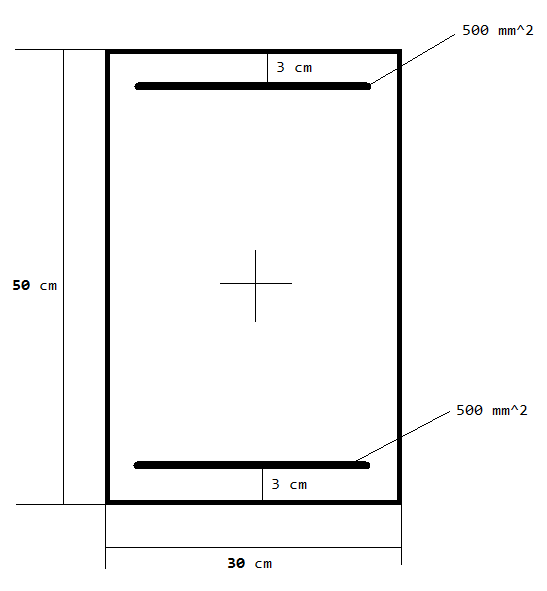
\includegraphics[width=0.5\textwidth]{img/pilastro30x50.png}
\caption{\footnotesize Pilastro $30 \times 50 \; cm$.}
\end{figure}
\textcolor{red}{migliorare immagine}

%\begin{table}[H]
%\begin{tabular}{c|ccccc}
% & \textbf{VcaSLU} & \textbf{EC2} & \texttt{\textbf{MchiNstrisce}} & \textbf{\texttt{MchiNstrisce}} & \textbf{\texttt{MchiN}} \\
% &  &  & yieldingPoint & findPoints2  & Analitico \\
% &  &  & ultimatePoint &   &  \\
%\hline
%$M_u$    & 0.092  & \\
%$\phi_u$ & 0.1134 & \\
%$y_u$    & \\
%\hline  
%$M_y$    & \\
%$\phi_y$ & \\
%$y_y$    & \\
%\end{tabular}
%\end{table}
%\textcolor{red}{invertire le righe con le colonne nella tabella?}

\begin{savenotes}

\begin{table}[H]
\centering
\begin{tabular}{l|ccc|ccc}
 & $M_u$ [MNm] & $\phi_u$ [1/m] & $y_u$ [m] & $M_y$ [MNm] & $\phi_y$ [1/m] & $y_y$ [m] \\
\hline
\textbf{VcaSLU}                & 0.092 & 0.1134 & 0.029 & 0.088 & 0.005 & - \\
\textbf{EC2}                   & 0.092 & -      & 0.028 & -     & -     & - \\
\textbf{FranchinEEtb}		   & 0.093 & 0.135  & $\sim$0.03 & 0.089 & 0.006 & $\sim$0.09 \\
\textbf{FranchinEEtb}(anal)	   & 0.092 & 0.1336 & 0.021 & 0.089 & 0.005 & 0.081 \\
\textbf{\texttt{MchiNstrisce}} (1)\footnote{\texttt{yieldingPoints} e \texttt{ultimatePoints}} 
                               & 0.092 & 0.1207 & 0.029 & 0.082 & 0.005 & 0.088 \\
\textbf{\texttt{MchiNstrisce}} (2)\footnote{\texttt{findPoints2}} 
							   & 0.092 & 0.1206 & -     & 0.090 & 0.005 & - \\
\textbf{\texttt{MchiN}}(anal)  \footnote{Analitico} 
                               & \\
\end{tabular}
\caption{\footnotesize Risultati per il pilastro a sezione $30\times50 \; cm$ con $\nu = 0.0$.}
\end{table}

\end{savenotes}

\begin{table}[H]
\centering
\begin{tabular}{l|ccc|ccc}
 & $M_u$ [MNm] & $\phi_u$ [1/m] & $y_u$ [m] & $M_y$ [MNm] & $\phi_y$ [1/m] & $y_y$ [m] \\
\hline
\textbf{VcaSLU}                    & 0.322 & 0.0178 & 0.185 & 0.307 & 0.008 & - \\
\textbf{FranchinEEtb}              & 0.400 & 0.021  & $\sim$0.21 & 0.383 & 0.009 & $\sim$0.27 \\
\textbf{FranchinEEtb}(anal)        & 0.403 & 0.0187 & 0.188 & 0.414 & 0.008 & 0.204 \\
\textbf{\texttt{MchiNstrisce}} (1) & 0.321 & 0.0189 & 0.185 & 0.296 & 0.008 & 0.239 \\
\textbf{\texttt{MchiNstrisce}} (2) & 0.321 & 0.0185 & -     & 0.281 & 0.004 & - \\
\textbf{\texttt{MchiN}}(anal)      & \\
\end{tabular}
\caption{\footnotesize Risultati per il pilastro a sezione $30\times50 \; cm$ con $\nu = 0.3$.}
\end{table}

L'errore massimo è del 10\% sul valore di $M_y$, mentre $\phi_y$ presenta una variabilità anche del 50\%. Il valore del momento ultimo $M_u$ e della profondità dell'asse neutro nello stato ultimo $y_u$ sono sostanzialmente identici. Le differenze nella definizione del momento e della curvatura di snervamento sono imputabili al fatto che la routine \texttt{findPoints2} trova il punto di snervamento facendo un fit della curva con un modello bilineare. Nell'immagine seguente sono riportate le curve $M-\phi$ per la sezione in esame.

Le soluzioni analitiche trovate tramite il foglio di Excel del Professor Franchin ("\texttt{FranchinEEtoolbox.xlsx}") sono riferite ad una sezione con armatura semplice (solo uno strato di armatura inferiore). \textcolor{red}{il momento ultimo è  minore di quello di snervamento per il caso $\nu = 0.3$?}


\begin{figure}[H]
\centering
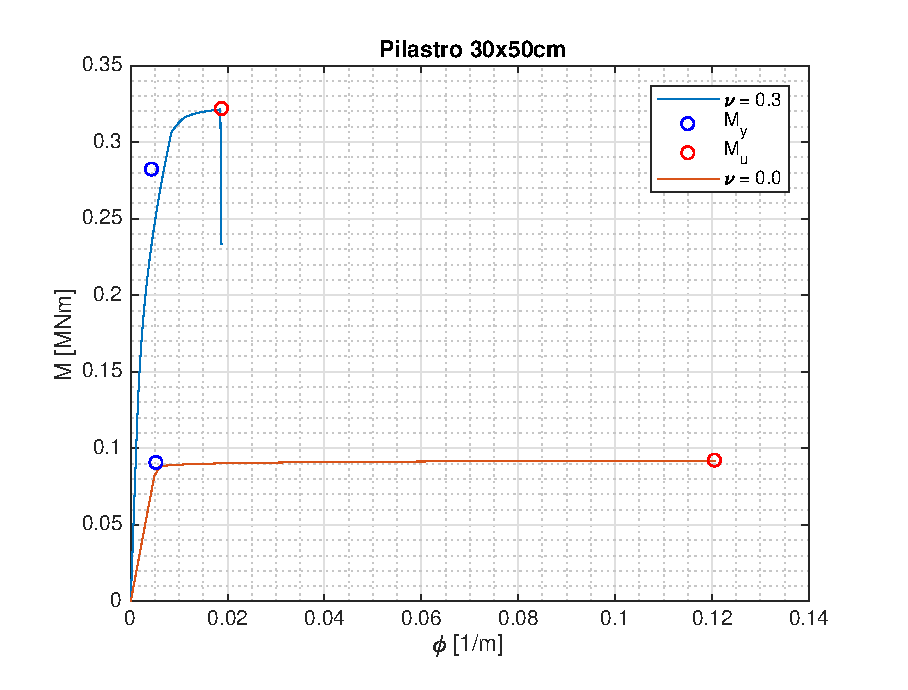
\includegraphics[width=0.8\textwidth]{img/pilastro30x50.eps}
\end{figure}




\subsection{Palo 120cm}

{\huge \textcolor{red}{PARE CHE CI SIA UNA DISCREPANZA TRA VCASLU E MCHIN (vedere i calcoli per il palo del Gatteo)}}

\begin{Large}
\textcolor{red}{Forse c'è un problema nel calcolo delle sezioni circolari...}
\end{Large}




\subsection{Pila 1250x1250x125}

\begin{figure}[H]
\centering
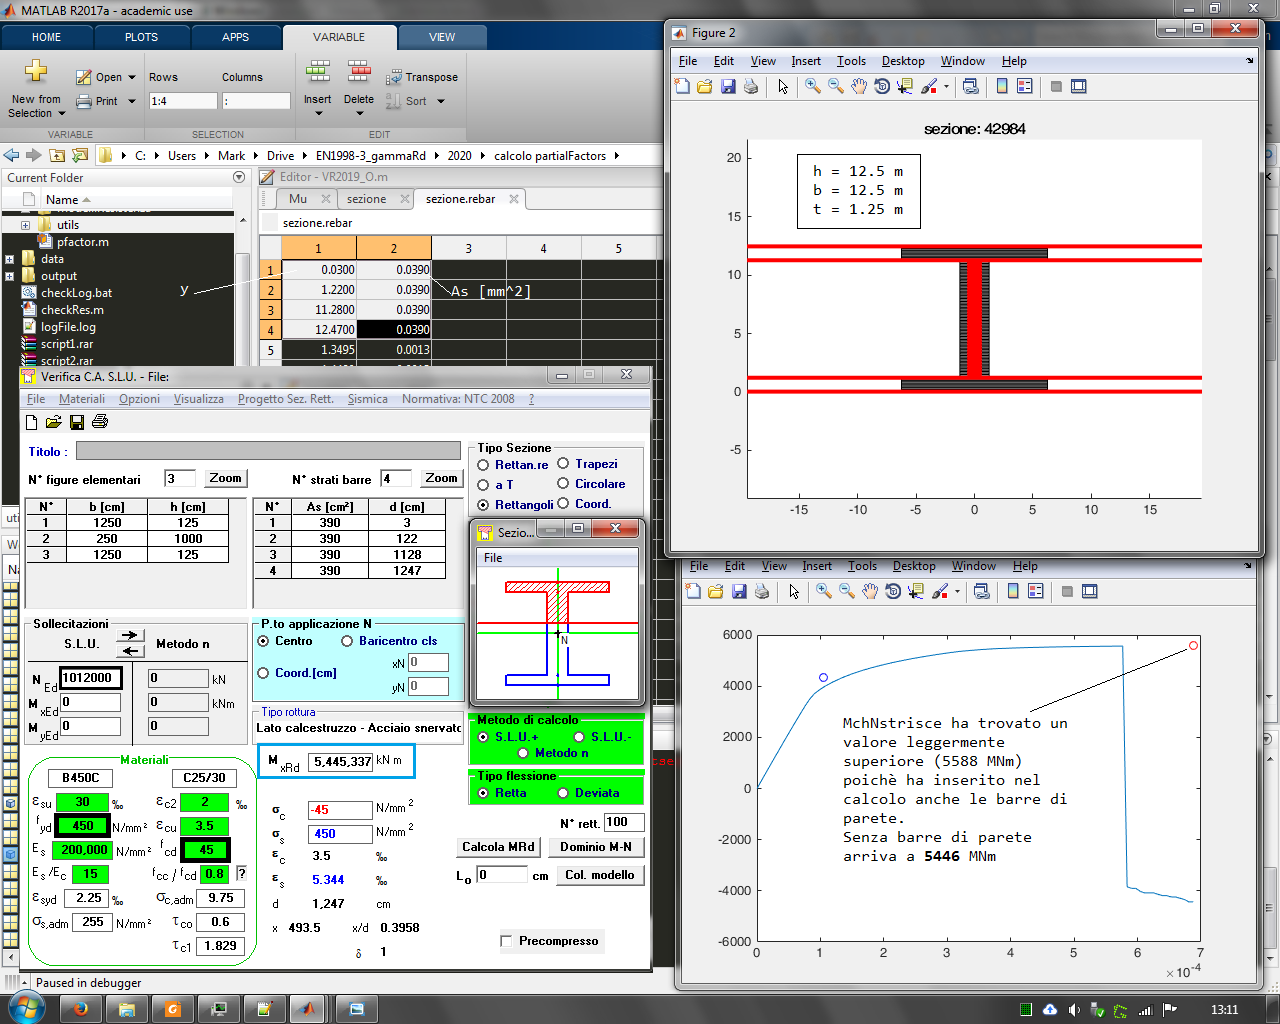
\includegraphics[width=\textwidth]{img/WIP109.png}
\end{figure}








\newpage

\section{Sezioni in acciaio}

In questa sezione vengono confrontati i risultati della routine \textit{MATLAB} "\texttt{MchiNstrisceSteel}" con i dati dei profilati ed altri software di analisi delle sezioni:
\begin{itemize}[noitemsep]
\item VcaSLU
\item EC2
\item SAP2000
\item \textcolor{gray}{SeRes}
\end{itemize}








\newpage

\appendix



\section{Esempio di utilizzo della classe}

Di seguito è riportato il codice per calcolare la sezione del pilastro 30x50 cm.

\begin{lstlisting}
%testa le procedure MchiN

addpath(genpath(pwd));


%% Pilastro 30x50cm

clc

%parametri
H  = 0.5;     %[m]
B  = 0.3;     %[m]
c  = 0.03;    %[m] (copriferro)
fc = 30;      %[MPa]
fy = 400;     %[MPa]
As = 500/1e6; %[m^2] (area di uno strato di armatura)
nu = 0.3;    %[-] (compressione normalizzata)
Nr = fc*H*B;  %[MN] (sforzo normale massimo)

disp('Pilastro 30x50cm');

sezione = MchiNstrisce(H/1000,@ParabRett,@ElastPlast);
sezione.defineMaterials(fc,fy,0.002,0.0035,0.002,0.06);
sezione.addLayer(H,B,B);
sezione.addRebar(c,As); %armatura inferiore
sezione.addRebar(H-c,As); %armatura superiore
sezione.initgeo;

N = - nu * Nr; %negativo: compressione

[M,phi,yn] = sezione.ultimatePoint(N);
disp('ultimatePoint:');
disp(['M_u   = ' num2str(M)]);
disp(['phi_u = ' num2str(phi)]);
disp(['yn_u  = ' num2str(yn)]);
[M,phi,yn] = sezione.yieldingPoint(N);
disp('yieldingPoint:');
disp(['M_y   = ' num2str(M)]);
disp(['phi_y = ' num2str(phi)]);
disp(['yn_y  = ' num2str(yn)]);

[My,chiy,Mu,chiu] = sezione.findPoints2(N,1);
disp('findPoints2:');
disp(['M_y   = ' num2str(My)]);
disp(['phi_y = ' num2str(chiy)]);
disp(['M_u   = ' num2str(Mu)]);
disp(['phi_u = ' num2str(chiu)]);
\end{lstlisting}



\newpage

\section{Programma \textit{MATLAB}}

\subsection{\texttt{MchiNstrisce.m}}

\begin{lstlisting}
% Questa classe e' basata sul codice SeReS_strisce

classdef MchiNstrisce < handle
    properties
        hmax %altezza massima del layer
        layer %matrice dove ogni riga e' un layer e le colonne sono: y, h, b_bot, b_top
        rebar %matrice dove ogni riga e' una barra e le colonne sono: y, As, mat_id
%         materials %struttura che contiene le funzioni sigma(eps) dei materiali (ogni riga e' un materiale differente)
        legameCLS %legame sigma(eps) del CLS
        legameAcc %legame sigma(eps) dell'acciaio
        %proprieta' aggiuntive:
        layersProp %ogni riga e' un layer, le colonne sono: Area, ygl
        %proprieta' dei materiali:
        fc %resistenza calcestruzzo
        fy %resistenza acciaio
        epscy, epscu %deformazione di snervamento e ultima del CLS
        epssy, epssu %deformazione di snervamento e ultima dell'acciaio
        %costanti della sezione:
        Area    %Area della Sezione
        yg      %coordinata del baricentro
        Ix      %Momento di inerzia secondo l'asse orizzontale
        H       %altezza totale della sezione
    end
    methods
        function obj = MchiNstrisce(hmax,CLS,Acc)
            %costruttore della classe
            obj.hmax = hmax;
            obj.legameCLS = CLS;
            obj.legameAcc = Acc;
        end
        
        function addLayer(obj,h,b,t)
            %aggiunge tanti layer alti massimo h_max fino a creare la patch
            %desiderata
            y = 0;
            for i=1:size(obj.layer,1); y = y + obj.layer(i,2); end
            sum = 0;
            while (h - (sum+obj.hmax) > 0)
                bj = b + (t-b)/(h)*(sum);
                tj = b + (t-b)/(h)*(sum+obj.hmax);
                if size(obj.layer,1) > 0; obj.layer = [obj.layer; (obj.layer(size(obj.layer,1),1)+obj.layer(size(obj.layer,1),2)) obj.hmax bj tj];
                else; obj.layer = [obj.layer; 0 obj.hmax b tj]; end %aggiunge il primo layer
                sum = sum + obj.hmax;
            end
            bj = b + (t-b)/(h)*(sum);
            if size(obj.layer,1) > 0; obj.layer = [obj.layer; (obj.layer(size(obj.layer,1),1)+obj.layer(size(obj.layer,1),2)) h-sum bj t];
            else; obj.layer = [obj.layer; 0 h b t]; end %aggiunge il primo layer
        end
        
        function addRebar(obj,y,As)
            %aggiunge uno strato di armature ordinarie
            obj.rebar = [obj.rebar; y As];
            
        end
        
        function defineMaterials(obj, fc, fy, eps_cy, eps_cu, eps_sy, eps_su)
            %aggiunge le proprieta' dei materiali
            if nargin < 4
                obj.fc = -abs(fc); %negativo: compressione
                obj.fy = fy;
                obj.epscy = -0.002; %negativo: accorciamento
                obj.epscu = -0.0035;
                obj.epssy = 0.002;
                obj.epssu = 0.03; %il massimo a cui sono arrivato e' il 6% (le NTC mi pare prescrivano l'1%)
            else
                obj.fc = -abs(fc);
                obj.fy = fy;
                obj.epscy = -abs(eps_cy);
                obj.epscu = -abs(eps_cu);
                obj.epssy = eps_sy;
                obj.epssu = eps_su;
            end
        end
        
        function initgeo(obj)
            %calcola la geometria della sezione
            %si prende in considerazione il fatto che sia composta tutta dello stesso materiale (in realta' dovrei SEMPRE omogeneizzare i layer [per ogni layer un coeff. di omogenizzazione n])
            obj.Area = 0;
            obj.Ix = 0;
            Sx = 0;
            for i=1:size(obj.layer,1)
                %1  2  3  4 
                %y, h, b, t, mat_id
                Areal = 0.5 * obj.layer(i,2) * (obj.layer(i,3) + obj.layer(i,4));
                ygl   = obj.layer(i,1) + obj.layer(i,2)/3 * (1+obj.layer(i,4)/(obj.layer(i,3)+obj.layer(i,4)));
                obj.Area = obj.Area + Areal;
                obj.layersProp = [obj.layersProp; Areal ygl];
                Sx = Sx + obj.layer(i,3) * obj.layer(i,2) * (obj.layer(i,2)/2 + obj.layer(i,1)) + 0.5*obj.layer(i,2)*(obj.layer(i,4)-obj.layer(i,3))*(2/3.*obj.layer(i,2) + obj.layer(i,1));
                obj.Ix = obj.Ix + 1/36*(obj.layer(i,2))^3*(2*obj.layer(i,3)+obj.layer(i,4)) + obj.layer(i,2)*(obj.layer(i,3)*(1/2*obj.layer(i,2)+obj.layer(i,1))^2 + 1/2*(obj.layer(i,4)-obj.layer(i,3))*(2/3*obj.layer(i,2)+obj.layer(i,1))^2);
            end
            obj.yg = Sx / obj.Area;
            obj.Ix = obj.Ix - obj.Area * (obj.yg)^2;
            obj.H = sum(obj.layer(:,2));
        end
        
        function [N,M] = setStrain(obj,eps_b,eps_t)
            %calcola N e M impostata la deformazione al lembo inferiore
            %(eps_b) e al lembo superiore (eps_t)
            
            %forze nei layers:
            Flayer = obj.legameCLS((eps_t-eps_b)*obj.layersProp(:,2)/obj.H+eps_b, obj.epscy,obj.epscu,obj.fc) .* obj.layersProp(:,1);
            %forze nelle barre:
            Frebar = obj.legameAcc((eps_t-eps_b)*obj.rebar(:,1)/obj.H+eps_b, obj.epssy,obj.epssu,obj.fy) .* obj.rebar(:,2);
            
            %contributo del calcestruzzo
            N = sum(Flayer);
            M = sum(Flayer .* obj.layersProp(:,2));
            %contrivuto dell'acciaio
            N = N + sum(Frebar);
            M = M + sum(Frebar .* obj.rebar(:,1));
            
            M = M - N * obj.yg; %aggiunge il momento dovuto alla forza normale
        end
        
        function [M,phi,yn] = yieldingPoint(obj, N)
            %calcola il punto di primo snervamento dato uno sforzo normale N
            % DA MIGLIORARE L'ALGORITMO!!!!!!! (vedi la procedura usata per
            % "ultimatePoint")
            
            if N < obj.fc*obj.Area; error('la sezione non puo' resistere a tale compressione'); end
            if N > obj.fy*sum(obj.rebar(:,2)); error('la sezione non puo' resistere a tale trazione'); end
            
            % fissato lo eps_inf = epssy cambia eps_top fino a trovare N corretto
            eps_inf = obj.epssy;
            
            %trova un range per fare la bisezione
            count = 0;
            eps_supP = obj.epssy; %l'ho scelto io (l'N iniziale puo' essere solamente minore)
            eps_supN = obj.epssy; %valore Negativo
            while obj.setStrain(eps_inf,eps_supN) > N
                eps_supN = eps_supN - 0.001;
                count = count + 1;
                if count > 1000; error('MchiNstrisce non e' arrivato a convergenza'); end
            end
            
            %fa la bisezione
            err = [100 100 100];
            count = 0;
            while ((abs(err(2)) > abs(0.005 * N)) )%|| (abs(eps_supP-eps_supN) > abs(0.0001*eps_supN))) %+0.000001 serve per non creare errori per N=0
                err = [(obj.setStrain(eps_inf,eps_supP) - N) (obj.setStrain(eps_inf,(eps_supP+eps_supN)/2) - N) (obj.setStrain(eps_inf,eps_supN) - N)];
                if err(1)*err(2) < 0
                    %la risultante e' tra err(1) e err(2) (eps_supP e' corretto)
                    eps_supN = (eps_supP+eps_supN)/2;
                    
                else
                    %la risultante e' tra err(2) e err(3) (eps_supN e' corretto)
                    eps_supP = (eps_supP+eps_supN)/2;
                end
                count = count + 1;
                if count > 1000; error('MchiNstrisce non e' arrivato a convergenza'); end
            end
            
            eps_sup = (eps_supP+eps_supN)/2;
            
            [~,M] = obj.setStrain(eps_inf,eps_sup);
            phi = (eps_inf-eps_sup)/obj.H; %compressione: negativa (la fibra superiore e' compressa)
            yn = -eps_sup/(eps_inf-eps_sup) * obj.H;
            M = -M; %convenzione italiana
        end
        
        function [M,phi,yn] = ultimatePoint(obj, N)
            %calcola il momento e la curvatura ultimi
            %il valore di N e' considerato negativo di compressione
            
            if N < obj.fc*obj.Area; error('la sezione non puo' resistere a tale compressione'); end
            if N > obj.fy*sum(obj.rebar(:,2)); error('la sezione non puo' resistere a tale trazione'); end
            
            %calcola lo sforzo normale interno della sezione nello stato di
            %rottura limite (armature a eps_su e calcestruzzo a eps_cu) e
            %se e' comunque minore dello sforzo agente N (quindi se la
            %sezione e' piu' compressa dello sforzo normale agente) vuol dire
            %che l'asse neutro deve "alzarsi" e quindi deve aumentare la
            %epsilon superiore (aumentare perche' prima era negativa:
            %-0.35%) Questo ultimo caso porta ad una rottura lato acciaio
            %(ovvero che e' fissa eps_inf e la bisezione si fa su eps_sup)
            if obj.setStrain(obj.epssu,obj.epscu) > N
                %si ha una rottura lato calcestruzzo, quindi e' tenuto fisso
                %eps_sup = eps_cu
                rottura_acciaio = 0;
                eps_sup = obj.epscu; %deformazione ultima del calcestruzzo (negativa: di accorciamento)
            else
                %si ha una rottura lato acciaio, quindi e' tenuto fisso
                %eps_inf = eps_su
                rottura_acciaio = 1;
                eps_inf = obj.epssu; %deformazione ultima dell'accaio (positiva: di allungamento)
            end
            
%             if rottura_acciaio; warning('rottura lato acciaio'); end
%             if rottura_acciaio; logFile('MchiN::ultimatePoint: rottura lato acciaio'); end
            
            
            %fa la bisezione
            err = [100 100 100]; %variabile di errore per la bisezione: [negativo, medio, positivo]
            count = 0;
            if rottura_acciaio == 0
                %rottura del CLS:
                eps_infP = obj.epssu; %deformazione ultima dell'acciaio (non puo' essere maggiore)
                eps_infN = obj.epscu; %deformazione ultima del calcestruzzo (non puo' essere minore)
                while ((abs(err(2)) > abs(0.0001 * N + 1e-18)) || (abs(eps_infP-eps_infN) > abs(0.0001*eps_infN))) %+1e-18 serve per non creare errori per N=0)
                    eps_infM = (eps_infP + eps_infN) / 2; %epsilon medio tra i due estremi (risparmio tre calcoli per ogni iterazione al costo di aggiungere una variabile)
                    err = [(obj.setStrain(eps_infN,eps_sup) - N) (obj.setStrain(eps_infM,eps_sup) - N) (obj.setStrain(eps_infP,eps_sup) - N)];
                    if err(2) > 0
                        %la risultante e' tra err(1) e err(2) (eps_infN e' corretto)
                        eps_infP = eps_infM;
                    else
                        %la risultante e' tra err(2) e err(3) (eps_infP e' corretto)
                        eps_infN = eps_infM;
                    end
                    count = count + 1;
                    if count > 10000; error('MchiNstrisce non e' arrivato a convergenza'); end
                end
                eps_inf = eps_infM;
            else
                %rottura dell'acciaio:
                eps_supP = 0; %potrebbe essere maggiore, potrebbe essere la deformazione di snervamento dell'acciaio
                eps_supN = obj.epscu; %deformazione ultima del calcestruzzo (non puo' essere minore)
                while ((abs(err(2)) > abs(0.0001 * N + 1e-18)) || (abs(eps_supP-eps_supN) > abs(0.0001*eps_supN))) %+1e-18 serve per non creare errori per N=0)
                    eps_supM = (eps_supP + eps_supN) / 2; %epsilon medio tra i due estremi (risparmio tre calcoli per ogni iterazione al costo di aggiungere una variabile)
                    err = [(obj.setStrain(eps_inf,eps_supN) - N) (obj.setStrain(eps_inf,eps_supM) - N) (obj.setStrain(eps_inf,eps_supP) - N)];
                    if err(2) > 0
                        %la risultante e' tra err(1) e err(2) (eps_supN e' corretto)
                        eps_supP = eps_supM;
                    else
                        %la risultante e' tra err(2) e err(3) (eps_supP e' corretto)
                        eps_supN = eps_supM;
                    end
                    count = count + 1;
                    if count > 9000
                        disp('sta per fallire');
                    end
                    if count > 10000; error('MchiNstrisce non e' arrivato a convergenza'); end
                end
                eps_sup = eps_supM;
            end
            
            [~,M] = obj.setStrain(eps_inf,eps_sup);
            phi = (eps_inf-eps_sup)/obj.H; %compressione: negativa (la fibra superiore e' compressa) IN REALTa' e' IL CONTRARIO (NEGATIVA)
            yn = -eps_sup/(eps_inf-eps_sup) * obj.H; %yn definito partendo all'"alto"
            M = -M; %convenzione italiana
        end

        
        function eps = deformazione(obj,eps0,chi,y)
            %funzione di epsilon: def(eps0,chi,y) = eps0 + chi*(y-yg)
            eps = eps0 + chi*(y-obj.yg);
        end
        
        function [f] = F(obj,eps0,chi,N0,M0)
            %calcola le funzioni
            %FUNZIONE AUSILIARIA
            [N,M]  = obj.Fint(eps0,chi);
            f(1,1) = N - N0;
            f(2,1) = M - M0;
        end
        
        function [N,M] = Fint(obj,eps0,chi)
            %restituisce le forze interne della sezione dato un profilo di
            %deformazione (definito da eps0 e chi)
 
            %----------------------------------------------------------
            %NUOVA FORMULAZIONE SENZA -yg NELLA FUNZIONE "deformazione"
            %----------------------------------------------------------
            
            N = sum(obj.legameCLS(obj.deformazione(eps0,chi,obj.layersProp(:,2)), obj.epscy,obj.epscu,obj.fc) .* obj.layersProp(:,1)) + ...
                sum(obj.legameAcc(obj.deformazione(eps0,chi,obj.rebar(:,1)), obj.epssy,obj.epssu,obj.fy) .* obj.rebar(:,2));
            M = sum(obj.legameCLS(obj.deformazione(eps0,chi,obj.layersProp(:,2)), obj.epscy,obj.epscu,obj.fc) .* (obj.layersProp(:,2)-obj.yg) .* obj.layersProp(:,1)) + ...
                sum(obj.legameAcc(obj.deformazione(eps0,chi,obj.rebar(:,1)), obj.epssy,obj.epssu,obj.fy) .* (obj.rebar(:,1)-obj.yg) .* obj.rebar(:,2));
        end
        
        function [M,chi] = curvaMchi3(obj,N,chi_lim)
            % calcola la curva M-chi-N
            %    inizialmente calcola i punti della curva con il metodo di
            %    Newton-Raphson e se fallisce calcola con la bisezione
            %    Con N=0 da problemi numerici, deve essere sempre <0
            
            if nargin < 3; chi_max = (obj.epssu-obj.epscu)/obj.H; else; chi_max = chi_lim; end
            
            N_punti = 100; %numero punti della curva
            delta = 1.e-12; %variazione per il calcolo numerico della derivata parziale
            tol = 1.e-8; %tolleranza per la convergenza (per il metodo di Newton)
            
            chi = linspace(0,chi_max,N_punti);
            M   = zeros(1,N_punti);
            
            for i=2:(N_punti) %parte da 2 perche' cosi' M(0) = 0 (altrimenti non lo e' per problemi numerici...)
                err   = 1; %variabile di errore (per il test di convergenza)
                eps0  = 0; %punto iniziale
                count = 0; %contatore che monitora il caso in cui va in loop infinito
                bisez = 0; %controlla se non bisogna ricorrere alla bisezione
                Nint  = 0;
                deltaNint = 100;
                while (err > tol) || (deltaNint > 0.001*abs(N))
                    Nint_old = Nint;
                    [Nint,~] = obj.Fint(eps0,chi(i));
                    deltaNint = abs(Nint-Nint_old);
                    derivata = (obj.Fint(eps0+delta,chi(i))-Nint)/delta;
                    eps0_old = eps0;
                    eps0 = eps0 + (1/derivata) * (N - Nint);
                    if eps0 ~= 0; err = abs((eps0 - eps0_old)/eps0); else; err = abs(eps0 - eps0_old); end
                    count = count + 1;
                    if count > 100 || derivata == 0
%                         warning('MchiN::curvaMchi2: Newton-Raphson non va bene, calcolo con la bisezione...');
                        logFile('MchiN::curvaMchi2: Newton-Raphson non va bene, calcolo con la bisezione...');
                        bisez = 1;
                        break;
                    end
                end
                if bisez
                    %cerca il range di laboro per la bisezione:
                    %fa la ricerca attraverso il "grid search"
                    for j=0:4
                        temp = linspace(-obj.epssu,obj.epssu,(2^j)*10);
                        Nint = zeros(size(temp));
                        for k=1:size(temp,2)
                            Nint(k) = obj.Fint(temp(k),chi(i));
                        end
                        [~,i_min] = min(Nint);
                        [~,i_max] = max(Nint);
                        if (Nint(i_min)<N && Nint(i_max)>N); break; end %ha trovato il range
                        %altrimenti continua finche' non e' discretizzato a
                        %sufficienza
                    end
                    if (Nint(i_min)>N || Nint(i_max)<N)
                        %se alla fine del for non ha ancora trovato il
                        %range allora non ci sono speranze neanche per la
                        %bisezione
%                         error('MchiN::curvaMchi2::bisezione: ERRORE nella ricerca del range per la bisezione');
                        %provare ad usare il "gradient descend" dal punto
                        %temp(i_min)
                        %IL TEST SULLA SEZIONE CIRCOLARE FALLISCE A QUESTO
                        %PUNTO PER \nu=0.3
                        M(i) = 0;
                        return;
                    end
                    eps0_min = temp(i_min);
                    eps0_max = temp(i_max);
                    
                    %esegue la bisezione:
                    count = 0;
                    Ntot = [1 1 1];
                    tol_bis = 0.00001; %tolleranza per la bisezione
                    while (norm(Ntot) > (tol_bis * abs(N))) || (abs(abs(eps0_max)-abs(eps0_min)) > (tol_bis * abs(eps0_min)))
                        eps0 = (eps0_min + eps0_max) / 2; %valore medio
                        Ntot(1) = obj.Fint(eps0_min,chi(i)) - N;
                        Ntot(2) = obj.Fint(eps0,chi(i)) - N;
                        Ntot(3) = obj.Fint(eps0_max,chi(i)) - N;
                        if (Ntot(1)*Ntot(2)) < 0
                            eps0_max = eps0;
                        else
                            eps0_min = eps0;
                        end
                        count = count + 1;
                        if count > 100
                            logFile('MchiN::curvaMchi2::bisezione: ERRORE convergenza');
                            error('MchiN::curvaMchi2::bisezione: non e' arrivato a convergenza');
                        end
                    end
                end
                [~,M(i)] = obj.Fint(eps0,chi(i));
            end
        end
        
        function [My,chiy,Mu,chiu] = findPoints(obj, N, ~)
            %trova i punti di snervamento e ultimo della sezione dalla
            %curva curvatura-momento.
            
            [~,chi_max] = obj.ultimatePoint(N); %METODO PER STABILIZZARE I RISULTATI NUMERICI
            [M,chi] = obj.curvaMchi3(N,chi_max); %calcola la curva "grezza"
            
            %trova il punto ultimo come il punto in cui la curva comincia
            %ad avere la derivata negativa (i materiali non hanno tratti
            %degradanti a tangente negativa):
%             i = find(diff(M) < 0 ,1); %tronca quando comincia a decrescere CERTE VOLTE FALLISCE PER PROBLEMI NUMERICI ALL'INIZIO
            [~,i] = max(M); %tronca quando raggiunge il massimo
            Mu   = M(i);
            chiu = chi(i);
            %elimina la parte di curva dopo il punto ultimo:
            M   = M(1:i);
            chi = chi(1:i);
            
            %trova il punto di snervamento bilinearizzando la curva:
            P0 = [chiu/3 3/4*Mu]; %parametri iniziali di prova
            model = @(P,x) (P(2)/P(1)*x).*heaviside(P(1)-x) + ((Mu-P(2))/(chiu-P(1))*(x-P(1))+P(2)).*heaviside(x-P(1)); %crea il modello da fittare
            lb = [0 0]; %lower bound (non ci possono essere valori negativi)
            ub = [chiu Mu]; %upper bound (il punto di snervamento non puo' essere maggiore di quello ultimo)
            options = optimoptions('lsqcurvefit','Display','off');
            Pfit = lsqcurvefit(model,P0,chi,M,lb,ub,options); %fitta il modello minimizzando i quadrati
            chiy = Pfit(1);
            My   = Pfit(2);
            
            %controlla i risultati:
            
            %comandi per i test:
            if nargin > 2
                plot(chi,M); hold on;
                plot(linspace(0,chiu,100),model(Pfit,linspace(0,chiu,100)),'k--');
                plot(chiy,My,'bo');
                plot(chiu,Mu,'ro');
            end
            
        end
        
        function [My,chiy,Mu,chiu] = findPoints2(obj, N, ~)
            %trova i punti trovando prima chi_u e poi discretizzando la
            %curva in un numero fisso di punti
            
            [Mu,chiu] = obj.ultimatePoint(N);
            [M,chi] = obj.curvaMchi3(N,chiu); %calcola la curva
            
            %trova il punto di snervamento bilinearizzando la curva:
            P0 = [chiu/3 3/4*Mu]; %parametri iniziali di prova
            model = @(P,x) (P(2)/P(1)*x).*heaviside(P(1)-x) + ((Mu-P(2))/(chiu-P(1))*(x-P(1))+P(2)).*heaviside(x-P(1)); %crea il modello da fittare
            lb = [0 0]; %lower bound (non ci possono essere valori negativi)
            ub = [chiu Mu]; %upper bound (il punto di snervamento non puo' essere maggiore di quello ultimo)
            options = optimoptions('lsqcurvefit','Display','off');
            Pfit = lsqcurvefit(model,P0,chi,M,lb,ub,options); %fitta il modello minimizzando i quadrati
            chiy = Pfit(1);
            My   = Pfit(2);
            
            %DEBUGGING
            if nargin > 2
                plot(chi,M); hold on;
                plot(chiy,My,'ob');
                plot(chiu,Mu,'or');
            end
            
        end
        
        function out = test(obj,eps0,chi)
            %esegue dei test sulla sezione
            
            N = zeros(size(eps0));
            M = zeros(size(eps0));
            
            for i=1:size(eps0,2)
                [N(i),M(i)] = obj.Fint(eps0(1,i),chi);
            end
            
            out(:,1) = N;
            out(:,2) = M;
            
        end
        
        function initRect(obj,h,b,As1,As2,c)
            %inizializza una sezione rettangolare
            if nargin < 6; c = 0.03; end
            obj.addLayer(h,b,b); %crea la sezione in CLS
            obj.addRebar(c,As1);
            obj.addRebar(h-c,As2);
            
            obj.initgeo;
        end
        
        function initRect2(obj,h,b,rhotot,rhoc_rhotot,db,c)
            %inizializza una sezione rettangolare (con anche l'armatura di parete)
            if nargin < 7; c = 0.03; end
            Ac = b*h; %area calcestruzzo
            Ab = pi/4 * db^2; %area della barra
            np = max(round((h-2*c)/0.3-1), 0); %calcola il numero di armature di parete (non ci puo' essere in interferro maggiore di 30 cm tra esse) [maggiore uguale a zero..]
            n2 = round(Ac*rhotot/Ab * rhoc_rhotot); %calcola il numero di armature superiori (compresse)            
            n1 = round(Ac*rhotot/Ab - n2 - 2*np);  %calcola il numero di armature inferiori (tese)
            
            obj.addLayer(h,b,b); %crea la sezione in CLS
            obj.addRebar(c,n1*Ab); %crea l'armatura inferiore
            obj.addRebar(h-c,n2*Ab); %crea l'armatura superiore
            %aggiunge le armature di parete:
            if np > 0
                interferro_laterale = (h-2*c)/(np+1);
                y = c + interferro_laterale;
                for i=1:np
                    obj.addRebar(y,2*Ab);
                    y = y + interferro_laterale;
                end
            end
            
            obj.initgeo; %calcola la geometria della sezione
        end
        
        function initCirc(obj,D,db,rhotot,c)
            %inizializza una sezione circolare
            if nargin < 6; c = 0.03; end
            AreaBarra = pi/4 * db^2;
            numeroBarre = round(rhotot * (D^2)/(db^2));
            
            hs = D/50;
            
            for y=linspace(0,D-hs,D/hs)
                thetab = acos(1 - 2/D*y);
                b = D*sin(thetab);
                thetat = acos(1 - 2/D*(y+hs));
                t = D*sin(thetat);
                obj.addLayer(hs,real(b),real(t));
            end
            for theta=linspace(0,pi,(numeroBarre+1)/2)
                y = D/2 - ((D-2*c)/2)*cos(theta);
                obj.addRebar(y,2*AreaBarra);
            end
            
            obj.initgeo;
        end
        
        function initHollow(obj,h,b,s,db,rhotot,c)
            %inizializza una sezione rettangolare cava
            if nargin < 7; c = 0.03; end
            AreaBarra = pi/4 * db^2;
            nBarre = round(rhotot*(8*s*(h+b-2*s))/(pi*db^2));
            interferro = 4*(h+b-2*s)/nBarre;
            nBarreParete = round(4*(h-2*s)/interferro); %round(8/pi * ((h-2*s)*s)/(db^2));
            nBarreStrati = round((nBarre-nBarreParete)/4);
            
            %crea la sezione in CLS
            obj.addLayer(s,b,b);
            obj.addLayer(h-2*s,2*s,2*s);
            obj.addLayer(s,b,b);
            %aggiunge gli strati orizzontali
            obj.addRebar(c,AreaBarra*nBarreStrati);
            obj.addRebar(s-c,AreaBarra*nBarreStrati);
            obj.addRebar(h-s+c,AreaBarra*nBarreStrati);
            obj.addRebar(h-c,AreaBarra*nBarreStrati);
            %aggiunge gli strati verticali
            interferro_parete = (h-2*s)/(nBarreParete/4 + 1);
            y = s + interferro_parete;
            for i=1:(nBarreParete/4)
%                 obj.addRebar(s+(h-2*s)*(i/(nBarreParete/4)),4*AreaBarra);
                obj.addRebar(y,4*AreaBarra);
                y = y + interferro_parete;
            end
            
            obj.initgeo;
        end
        
        function plotSection(obj)
            %plotta la sezione
            
            for i=1:size(obj.layer,1)
                %plotta i layers
                y = obj.layer(i,1); %ordinata del lembo inferiore del layer
                h = obj.layer(i,2); %altezza del layer
                b = obj.layer(i,3); %larghezza di base del layer
                t = obj.layer(i,4); %larghezza superiore del layer
                Xp = [-b/2 b/2 t/2 -t/2];
                Yp = [y y y+h y+h];
                patch(Xp,Yp,[0.8 0.8 0.8]);
                hold on;
            end
            
            for i=1:size(obj.rebar,1)
                %plotta le barre
                y = obj.rebar(i,1);
                As = obj.rebar(i,2);
%                 line([-As/2*1000 As/2*1000],[y y],'Color','red');
                plot([-As/2*1000 As/2*1000],[y y],'r','LineWidth',3);
            end
			
			hold off;
%             text(0,obj.H/2,num2str(size(obj.rebar,1)));
            axis equal;
        end
        
        
    end
    
end



% ChangeLog:
% ----------
%   13/01/2021: Ho modificato le funzioni "ultimatePoint" eliminando la ricerca iniziale del range e "Fint" eliminando il -yg nel calcolo dellal deformazione
%   16/01/2021: Ho eliminato "findEquilibrium" e "curvaMchi" che non erano usate da tempo
%   17/01/2021: Ho inserito la funzione "curvaMchi3" che migliora "curvaMchi2"
%   
\end{lstlisting}


\subsection{Legami costitutivi}

\subsubsection{Calcestruzzo}

\begin{lstlisting}[caption=\footnotesize legame costitutivo parabola-rettangolo per il calcestruzzo armato (\texttt{ParabRett.m})]
function sigma = ParabRett(eps,epsy,epsu,smax)
    %legame costitutivo CLS NTC2018
    %eps e' negativo di compressione
    
%     epsy = -0.0020;
%     epsu = -0.0035;
%     smax = -30; %MPa
    
    sigma = zeros(size(eps));
    for i=1:size(eps)
        if (eps(i) > 0); sigma(i) = 0; %non resistente a trazione
        elseif (eps(i) >= epsy); 	sigma(i) = smax * (2*eps(i)/epsy - (eps(i)*eps(i))/(epsy*epsy));
        elseif (eps(i) >= epsu); 	sigma(i) = smax;
        elseif (eps(i) < epsu);    sigma(i) = 0.0;
        end
    end
end
\end{lstlisting}

\begin{lstlisting}[caption=\footnotesize legame costitutivo parabola-rettangolo per il calcestruzzo armato con la definizione anche della resistenza a trazione (\texttt{ParabRett2.m})]

\end{lstlisting}



\subsubsection{Acciaio}

\begin{lstlisting}[caption=\footnotesize legame costitutivo elasto-plastico perfetto per l'acciaio (\texttt{ElaspPlast.m})]
function sigma = ElastPlast(eps,epsy,epsu,smax)
    %legame costitutivo elastoplastico perfetto
    
%     %acciaio B450C (NTC2018):
%     epsy = 0.002;
%     epsu = 0.010;
%     smax = 391; %MPa
    
    sigma = zeros(size(eps));
    for i=1:size(eps)
        if (eps(i) <= -epsu);		sigma(i) = 0.0;
        elseif (eps(i) <= -epsy);	sigma(i) = -smax;
        elseif (eps(i) <= epsy); 	sigma(i) = eps(i) * (smax/epsy); 
        elseif (eps(i) <= epsu); 	sigma(i) = smax; 
        elseif (eps(i) > epsu); 	sigma(i) = 0.0;
        end
    end
end
\end{lstlisting}







\end{document}